\documentclass{beamer} 
\usepackage{listings}
\usepackage{amsmath}
\usepackage[absolute,overlay]{textpos}
\hypersetup{ colorlinks, citecolor=blue, linkcolor=red}
\usetheme{boxes}
\setbeamercovered{invisible}
\usecolortheme{crane}
\setbeamertemplate{navigation symbols}{}
\usepackage{graphicx}
\beamertemplatenavigationsymbolsempty
\setbeamerfont{page number in head/foot}{}
\setbeamertemplate{footline}[frame number]

\logo{

\includegraphics[height=1cm]{../fig/mfrc}
%\hspace{10.2cm}
%
\includegraphics[height=1.0cm]{../fig/gmit}
} 
\title[olga.lyashevska@gmit.ie]{How can machine learning help to predict changes in size of Atlantic herring?}
\author[Lyashevska et al, 2016]{
Olga Lyashevska$^{*}$ \and Clementine Harma \and Deirdre Brophy \and Coilin Minto \and Maurice Clarke}
\institute[] 
{
*    
Marine and Freshwater Research Centre\\
Galway-Mayo Institute of Technology (GMIT)\\
Galway, Ireland\\
\medskip {\emph{olga.lyashevska@gmit.ie}} } 


\date{July, 22 2016}

%in this talk I will present a supervised machine learning algorithm to identify drivers of change in  

\begin{document} 
\begin{frame} 
\titlepage 
\end{frame}

%\begin{frame}[allowframebreaks]
\begin{frame}
\frametitle{Background}

%There is a decline in size of Atlantic herring (\textit{Clupea harengus}) in the Celtic Sea.
%since the beginning of 1980's the size has decreased by approximately 4 cm

\begin{center}
{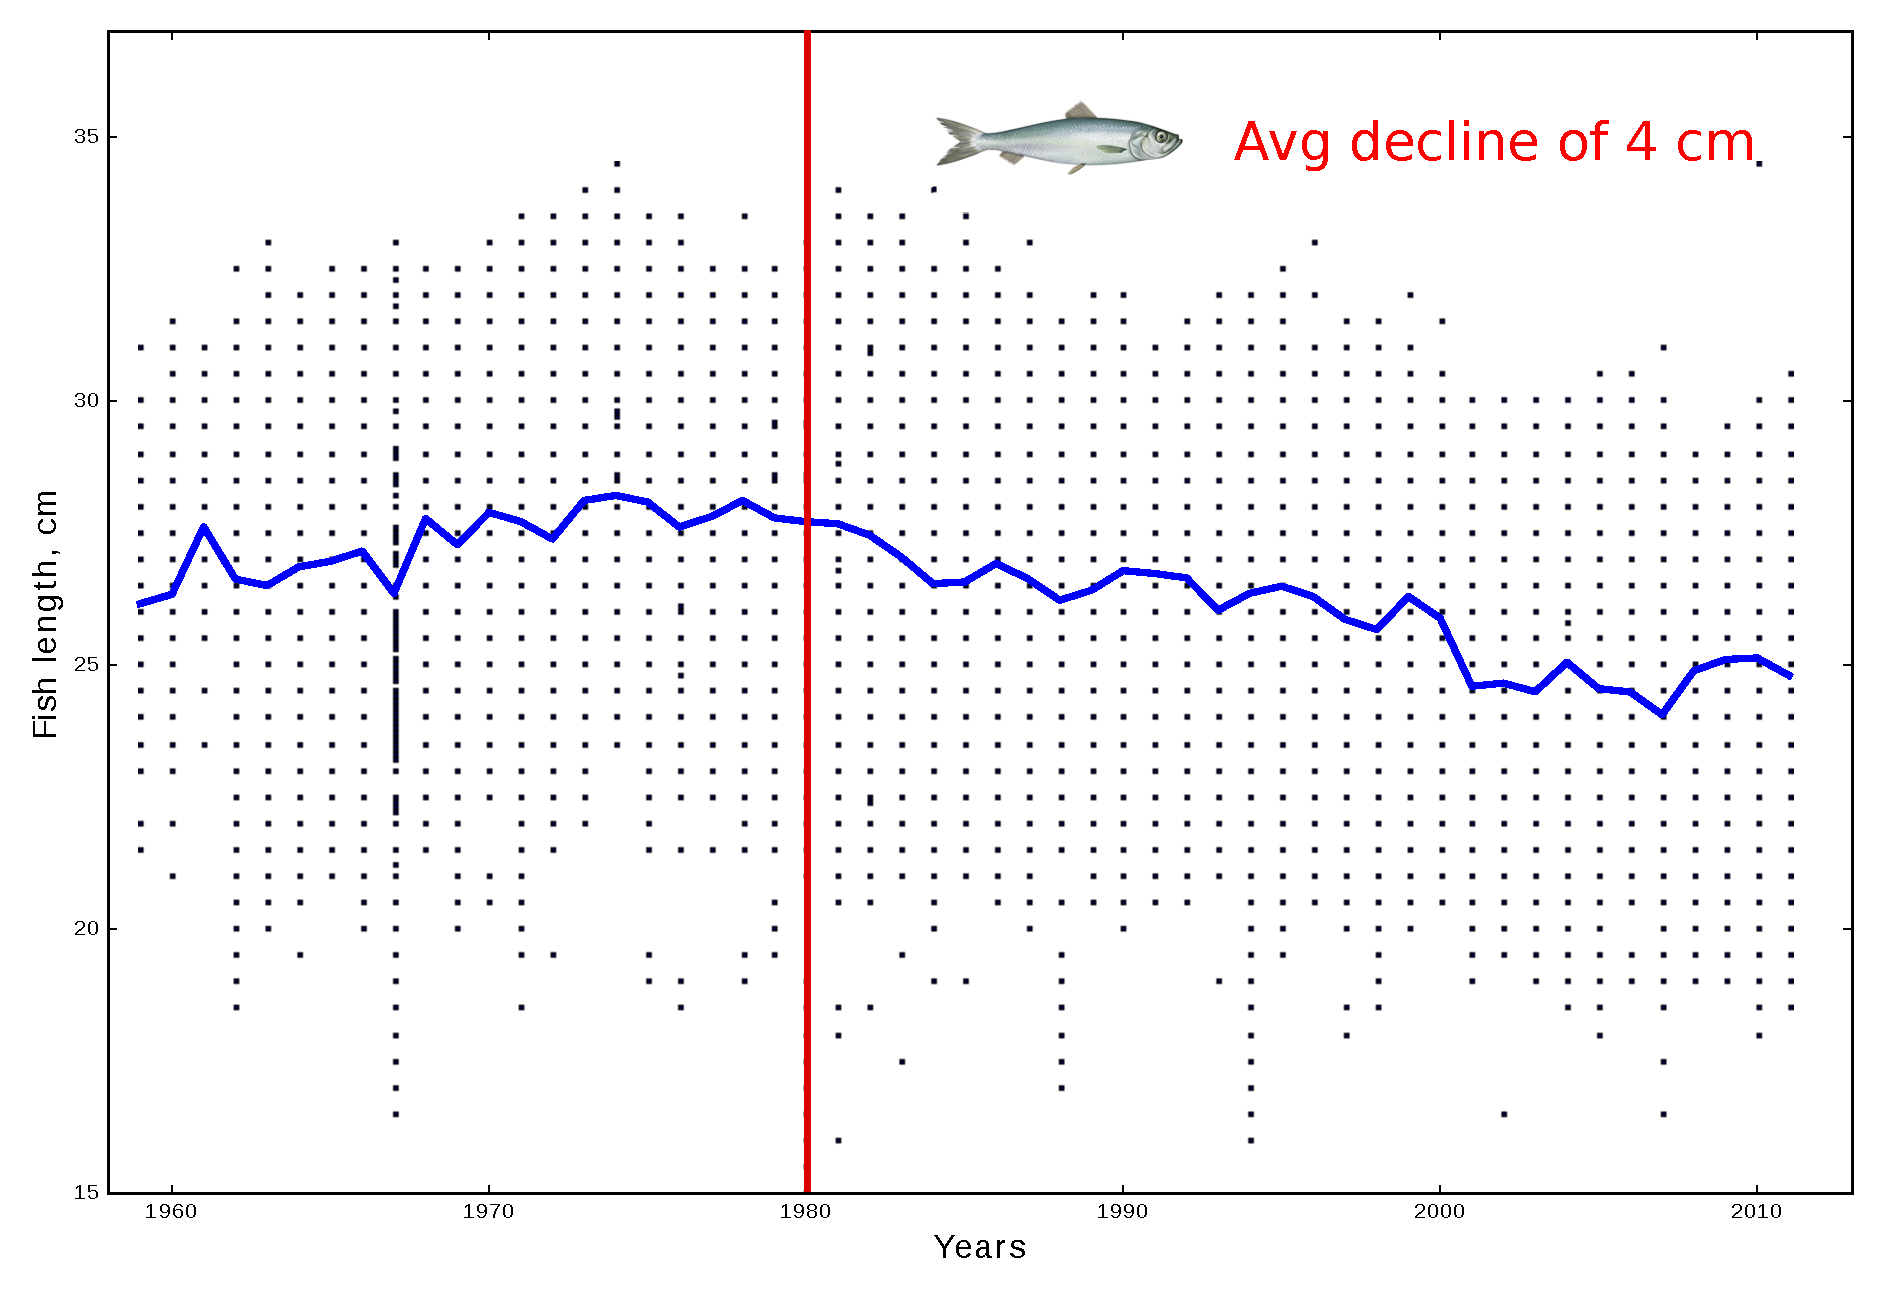
\includegraphics[scale=0.34]{../fig/fish-length} }
\end{center}
\end{frame}

\begin{frame} 
\frametitle{Problem}
\begin{itemize}
\item <+-| alert@+> Herring are one of the most important pelagic species exploited by fisheries;
\item <+-| alert@+> Reductions in growth have consequences for stock productivity;
\item <+-| alert@+> The cause of the decline remains largely unexplained;
 \item <+-| alert@+> Likely to be driven by the \textbf{interactive effect} of various factors:	
    \begin{itemize}
        \item sea surface temperature;
        \item zooplankton abundance; 
        \item fish abundance; 
        \item fishing pressure;
\end{itemize}
\end{itemize}
\end{frame} 


\begin{frame}
\frametitle{Data}
%A long time-series of biological data obtained from commercial landings
    \begin{itemize}
        \item 1959 -- 2012;
        \item throughout the year;
        \item random sampling (n = 50 to 100) from commercial vessels;
        \item pelagic trawling;
        \item age and weight-at-length;
        \item total sample size 50,000;
    \end{itemize}
\begin{center}
{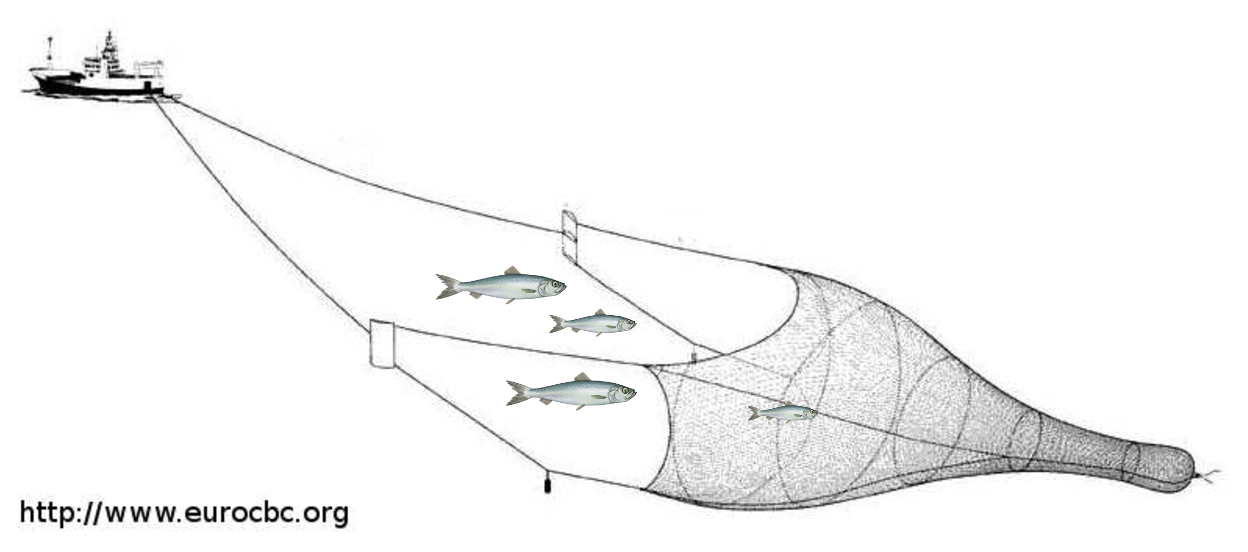
\includegraphics[scale=0.4]{../fig/trawl} }
\end{center}
        
\end{frame}

% The study area is the area of the Atlantic Ocean off the south coast of Ireland bounded to the east by Saint George's Channel; Bristol Channel and the English Channel

\begin{frame}
\frametitle{Study Area}
\begin{figure}
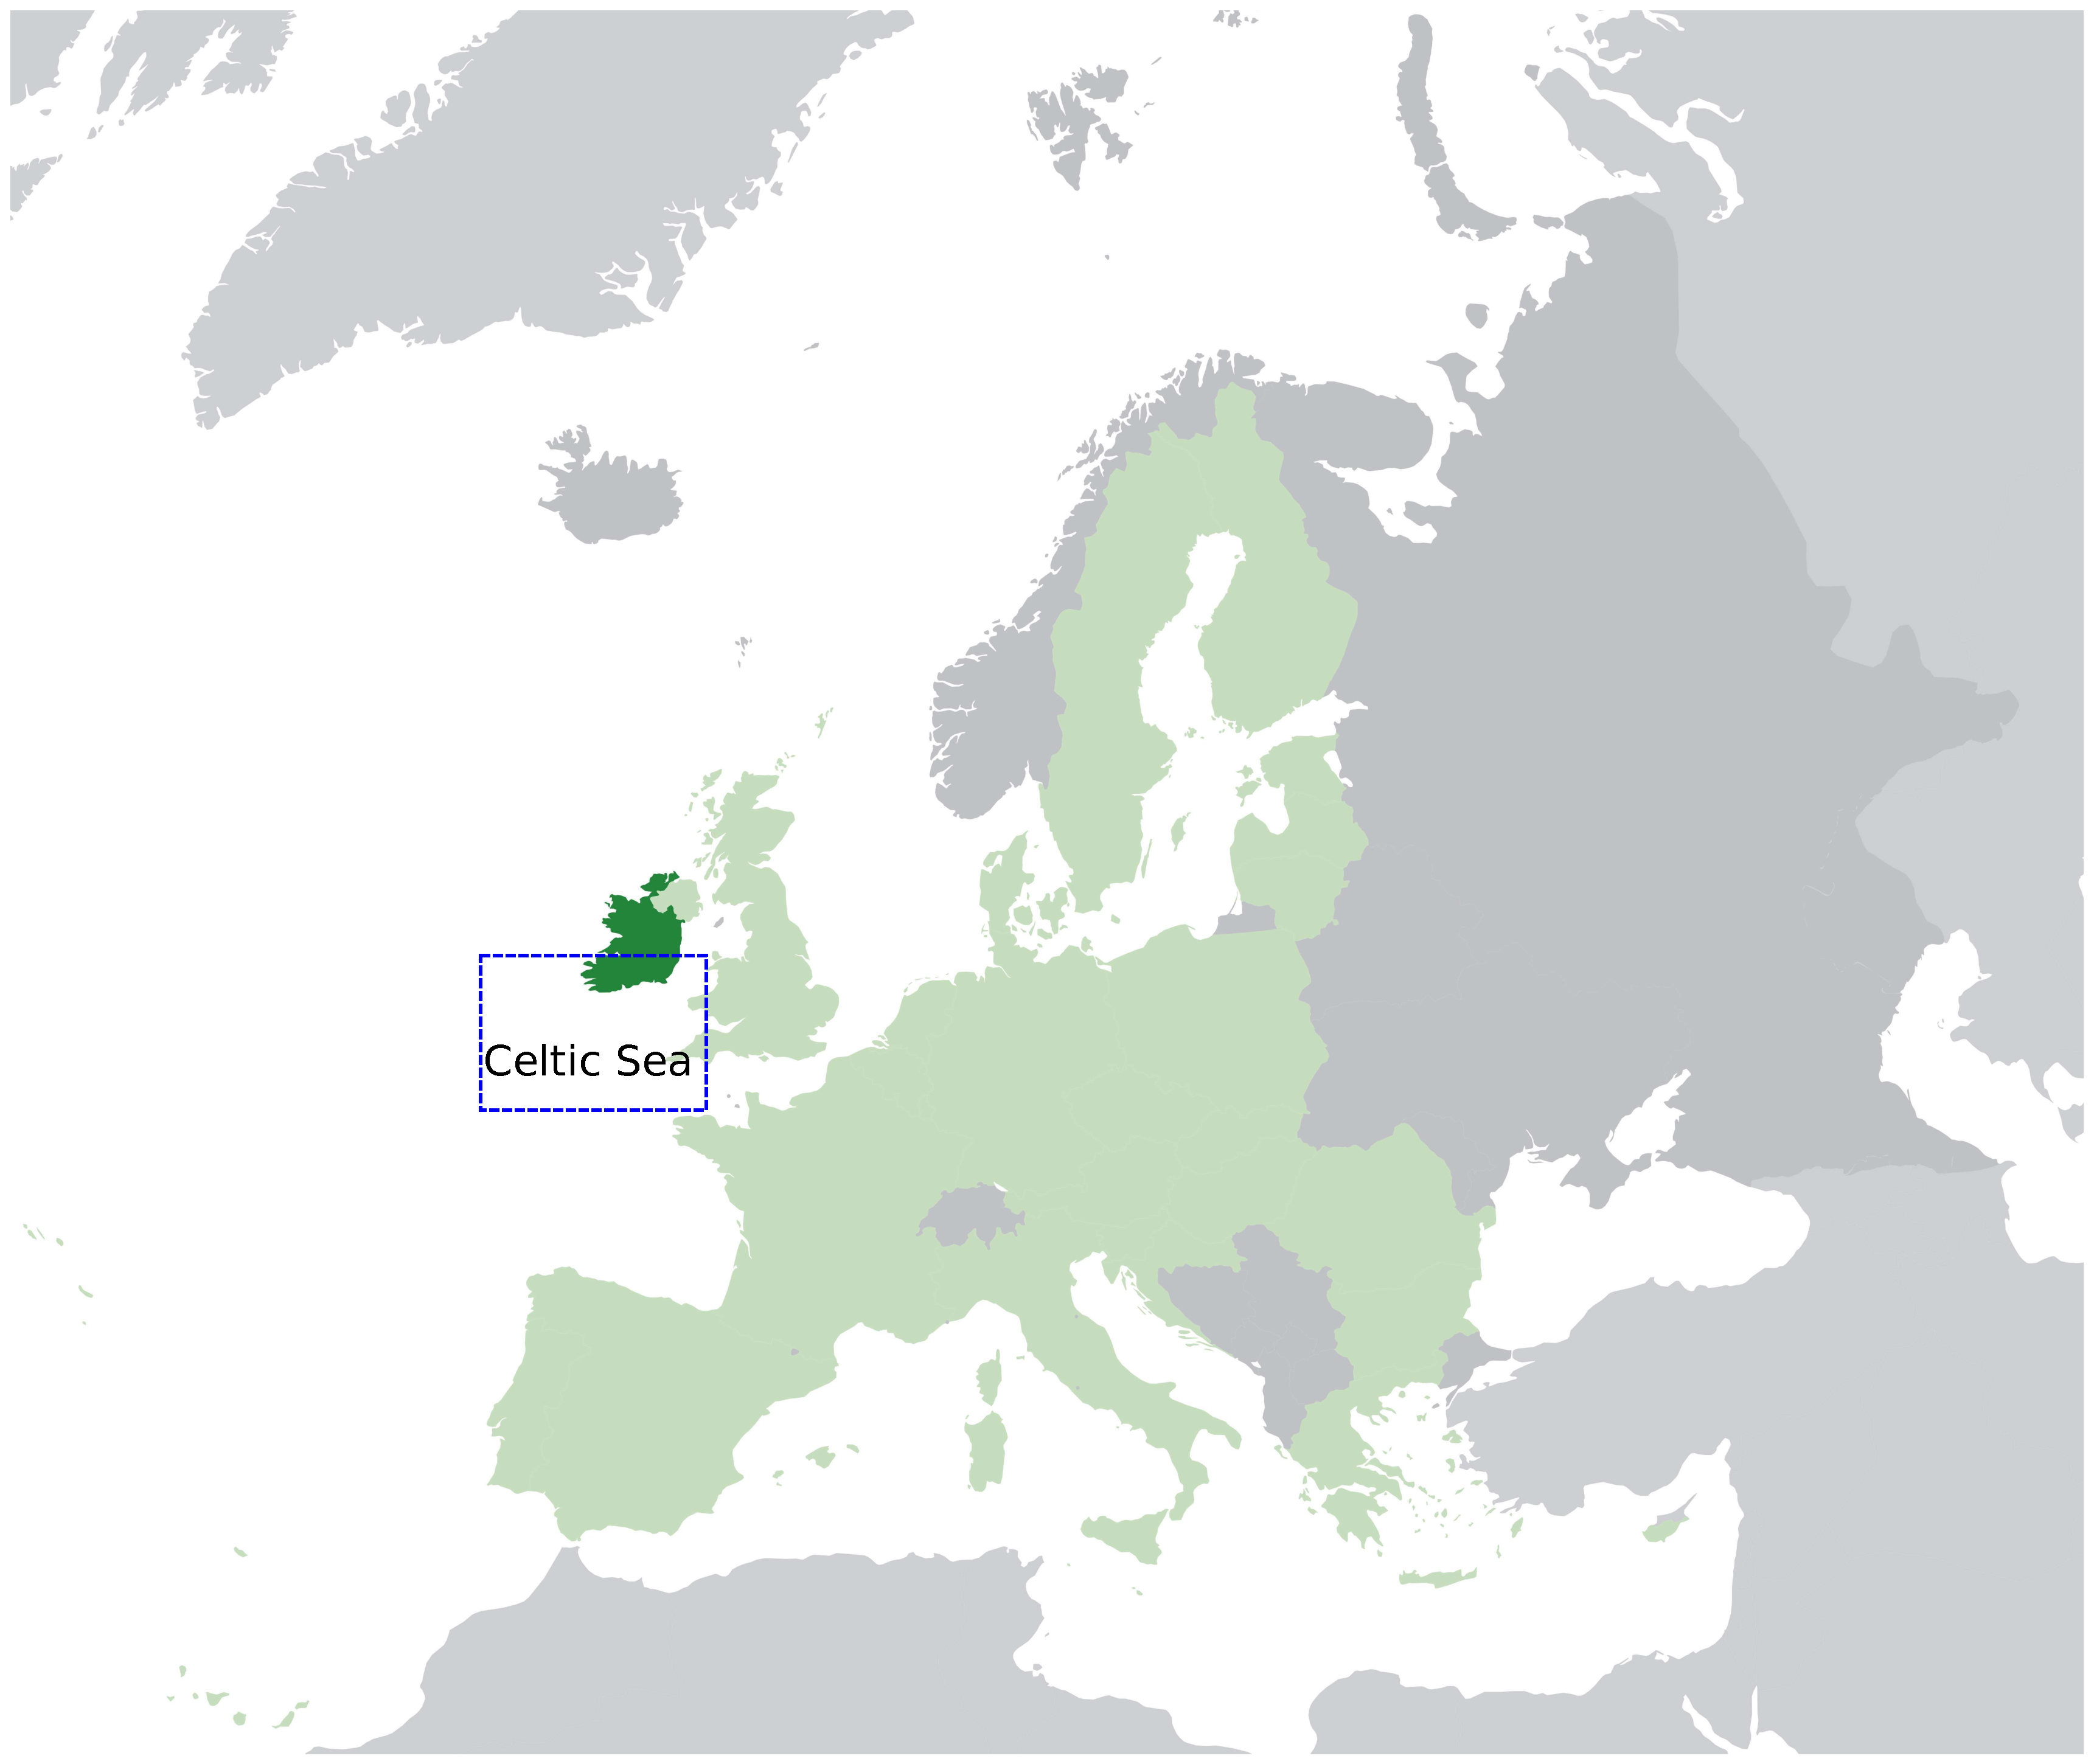
\includegraphics[width=1.1\linewidth,height=0.85\textheight,keepaspectratio]{../fig/EU-Ireland} 
\end{figure}
\end{frame}

%GBRT is a supervised machine learning algorithm which belongs to ensemble methods.
%ensemble is because we have not a single tree but a collection of regressian trees, called weak learners.
%weak learners because they are only slightly better than a random guess
%it works as following:
%Fit a sequence of weak learners on repeatedly reweighted versions of the data. The predictions are then combined through a weighted sum to produce the final prediction.
%because each consequent tree is based on the residuals of the previous, the accuracy of the single estimator is improved

%this is different from other ensemble methods, such as e.g. bagging or random forest, in which the driving principle is to build several estimators independently and then to average their predictions. The combined estimator is usually better than any of the single base estimators because its variance is reduced.
% in contrast in boosting, base estimators are built sequentially and the motivation is to combine several weak models to produce a powerful ensemble e.g. Ada Boost, Gradient Tree Boosting

\begin{frame}
\frametitle{Objective}
To identify important variables underlying changes in growth  using Gradient Boosting Regression Trees (GBRT)
\centering
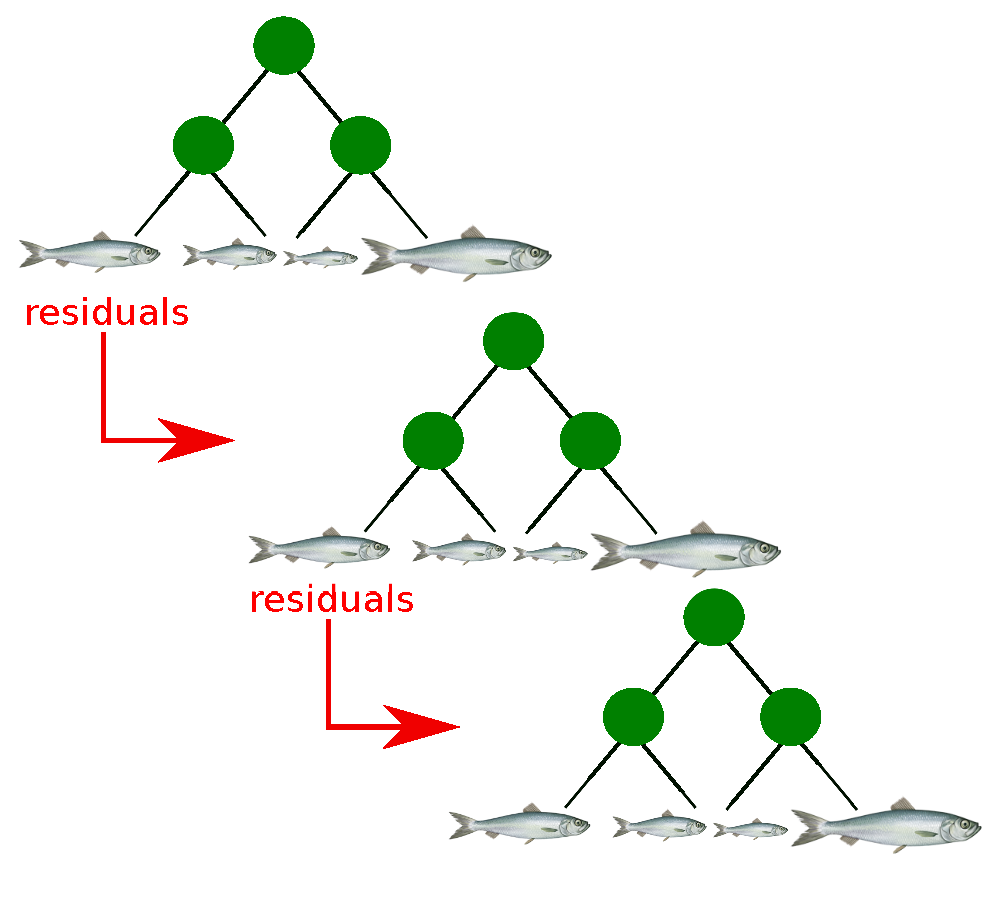
\includegraphics[scale=0.47]{../fig/herring-tree}
\end{frame}

\begin{frame}
\frametitle{GBRT} %all decision tree methods 
    \begin{itemize}
    \item <+-| alert@+> Advantages:
    \begin{itemize}
        \item Detection of (non-linear) feature interactions; 
        \item Resistance to inclusion of irrelevant features; %because they perform internal features selection as an integral part of the procedure 
        \item Heterogeneous data (features measured on different scale);
        \item Robustness to outliers;
        \item Accuracy; %improved in GBRT
        \item Different loss functions %in GBRT 
    \end{itemize}
    \item <+-| alert@+> Disdvantages:
    \begin{itemize}
        \item Requires careful tuning;
        \item Slow to train (but fast to predict);
    \end{itemize}
    \end{itemize}
\end{frame}

% formally:

\begin{frame}
    \frametitle{Formal Specification}
%GBRT considers additive models of the following form:
    \begin{equation}
    F_{m}(x) = \sum_{m=1}^{M}\gamma_{m}{h_{m}(x)}
    \end{equation}

    where $\gamma_{m}$ is a weight and $h_m(x)$ are weak learners.\\

\pause

GBRT builds the additive model in a forward stagewise fashion:

    \begin{equation}
    F_m(x) = F_{m-1}(x) + \epsilon \gamma_m h_m(x)
    \end{equation}

where $\epsilon$ is a shrinkage.  %scales the contribution of each weak learner by a factor, also called learning rate because it scales the step length of the gradient descent procedure;
\pause
    
    At each stage the weak learner $h_m(x)$ is chosen to minimize the loss function $L$ given the current model $F_{m-1}$ and its fit $F_{m-1}(x_i)$

    \begin{equation}
    F_m(x) = F_{m-1}(x) + \arg\min_{h} \sum_{i=1}^{n} L(y_i, F_{m-1}(x_i) - h(x))
    \end{equation}

% The minimization problem is solved numerically via steepest descent. 
% The direction of which is the negative gradient of the loss function evaluated at the current model $F_{m-1}$ which can be calculated for any differentiable loss function. I will not go into details of that.
\end{frame}

%\begin{frame}
%    \frametitle{Formal Specification}
%
%The minimization problem is sloved numerically via steepest descent. 
%The steepest descent direction is the negative gradient of the loss function evaluated at the current model $F_{m-1}$ which can be calculated for any differentiable loss function:
%
%    \begin{equation}
%    F_m(x) = F_{m-1}(x) + \gamma_m \sum_{i=1}^{n} \nabla_F L(y_i, F_{m-1}(x_i))
%    \end{equation}
%
%\pause
%
%Where the step length $\gamma_m$ is chosen using line search:
%
%    \begin{equation}
%    \gamma_m = \arg\min_{\gamma} \sum_{i=1}^{n} L(y_i, F_{m-1}(x_i) - \gamma \frac{\partial L(y_i, F_{m-1}(x_i))}{\partial F_{m-1}(x_i)})
%    \end{equation}
%\end{frame}
%

%the most important parameters
% must be tuned
% the parameters were optimised by cross-validated grid-search over a parameter grid

\begin{frame}
    \frametitle{GBRT hyperparameters}
    \begin{itemize}
% n_estimators and learning_rate are two regularisation parameters, each one control the degree of fit, and thus the best value for the other one
        \item \alert{number of iterations  = 500; }
%number of weak learners
% this parameter strongly interacts with the learning rate
% Smaller values of learning_rate require larger numbers of weak learners to maintain a constant training error. 
% Empirical evidence suggests that small values of learning_rate favor better test error. 
% hastie2009 suggests to set the learning rate to a small constant (e.g. learning_rate <= 0.1) and choose n_estimators by early stopping. 
        \item \alert{shrinkage (learning rate) = 0.05; }
%The parameter \nu is also called the learning rate because it scales the step length the the gradient descent procedure
        \item max tree depth = 6; 
% the degree of feature interaction
%Work best with shallow decision trees = weak models
%The size of the regression tree base learners defines the level of variable interactions that can be captured by the gradient boosting model. 
 %In general, a tree of depth 4 can capture interactions of order 3. 
        \item subsample = 0.75; 
% introduces stochasticity
%at each iteration the weak learner is trained on a fraction subsample of the available training data %the fraction of samples to be used for fitting the individual base learners, <1.0 leads to reduction of variance and an increase in bias
% in a way stochastic gradient boosting combines gradient boosting with bootstrap averaging (bagging)
        \item loss function = Least Squares; 
%The natural choice for regression due to its superior computational properties. The initial model is given by the mean of the target values.
% the other possibilities are least absolute deviation or huber, that combines both ls and lad
    \end{itemize}
    \vspace{1cm}
    \raisebox{-0.35ex}{
\includegraphics[width=10.5ex]{../fig/python}} \qquad
    \raisebox{-0.35ex}{
\includegraphics[width=6.5ex]{../fig/scikit-learn}}%
    %\citep{scikit-learn}
\end{frame}

% train and test error at each iteration
% closely follow each other, suggesting that the model was tuned properly 
% Plots like these can be used to determine the optimal number of trees by early stopping
% mse levels off

\begin{frame}
\frametitle{Model estimation}
    \vspace{-1cm}
\begin{columns}[c]    
\column{.65\textwidth}
    \centering
\begin{figure}
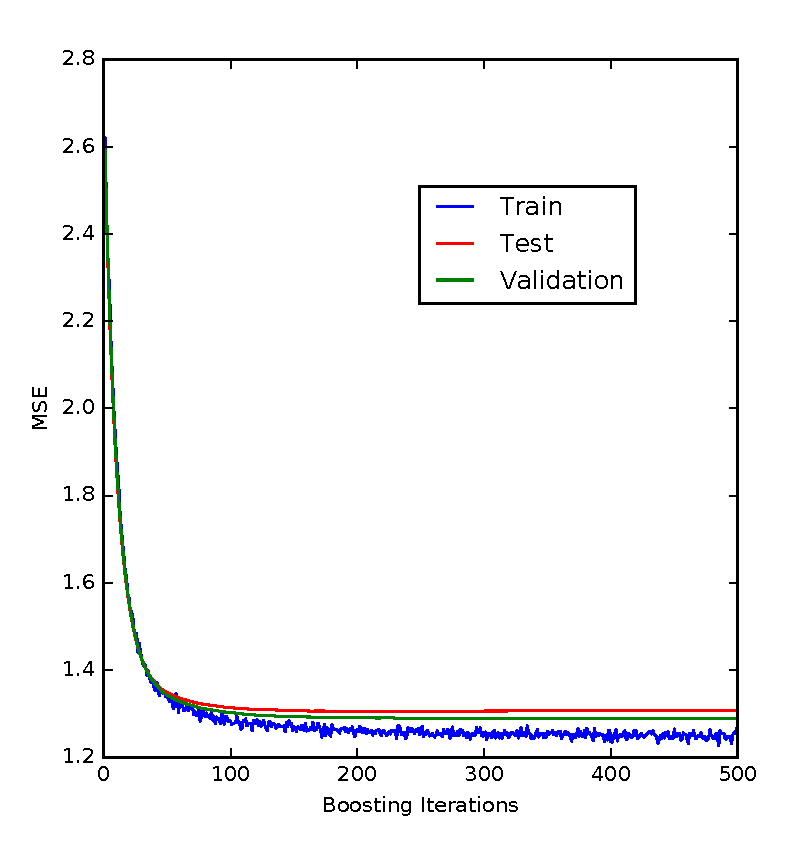
\includegraphics[scale=0.55]{../fig/devianceCS-present}
\end{figure}
\column{.35\textwidth}
  \centering
  \begin{itemize}
      \item MSE: 1.31
      \item $R^2$ train: 54.5\%
      \item $R^2$ test: 51.7\%
      \item $R^2$ val: 52.6\%
  \end{itemize}
\end{columns}
\centering Low $R^2$ due to individual variability 
\end{frame}


% When interpreting a model, the first question usually is: what are those important features and how do they contributing in predicting the target response?
% Often features do not contribute equally to predict the target response; in many situations the majority of the features are in fact irrelevant. 

% any regression trees method intrinsically perform feature selection by selecting appropriate split points. 
% This information can be used to measure the importance of each feature; the basic idea is: the more often a feature is used in the split points of a tree the more important that feature is. 
% This notion of importance can be extended to decision tree ensembles by simply averaging the feature importance of each tree

\begin{frame}
    \frametitle{True vs Predicted}
\begin{figure}
    \centering
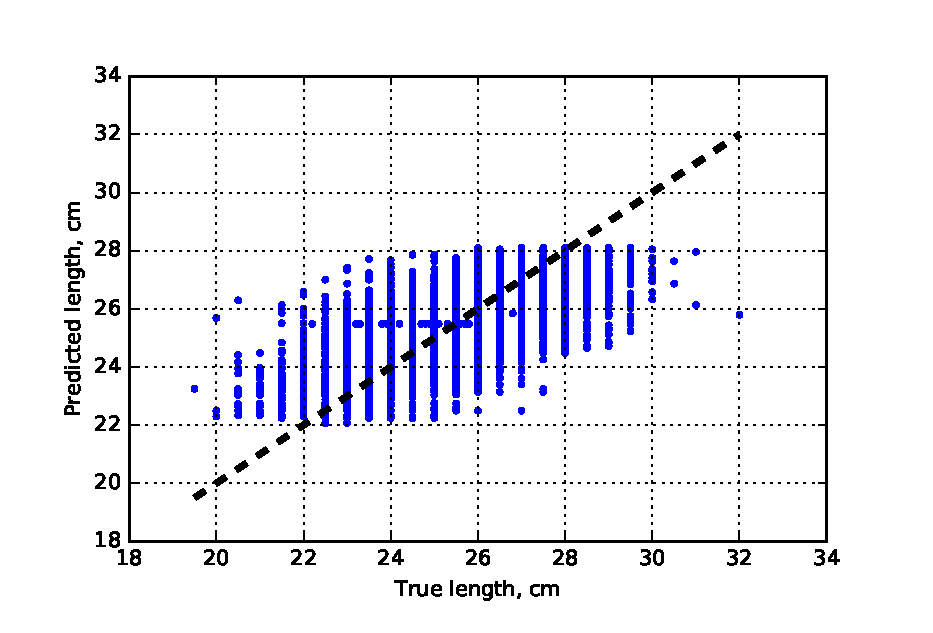
\includegraphics[scale=0.75]{../fig/true-pred-present}
\end{figure}
\end{frame}



\begin{frame}
    \frametitle{Variable Importance Plot}
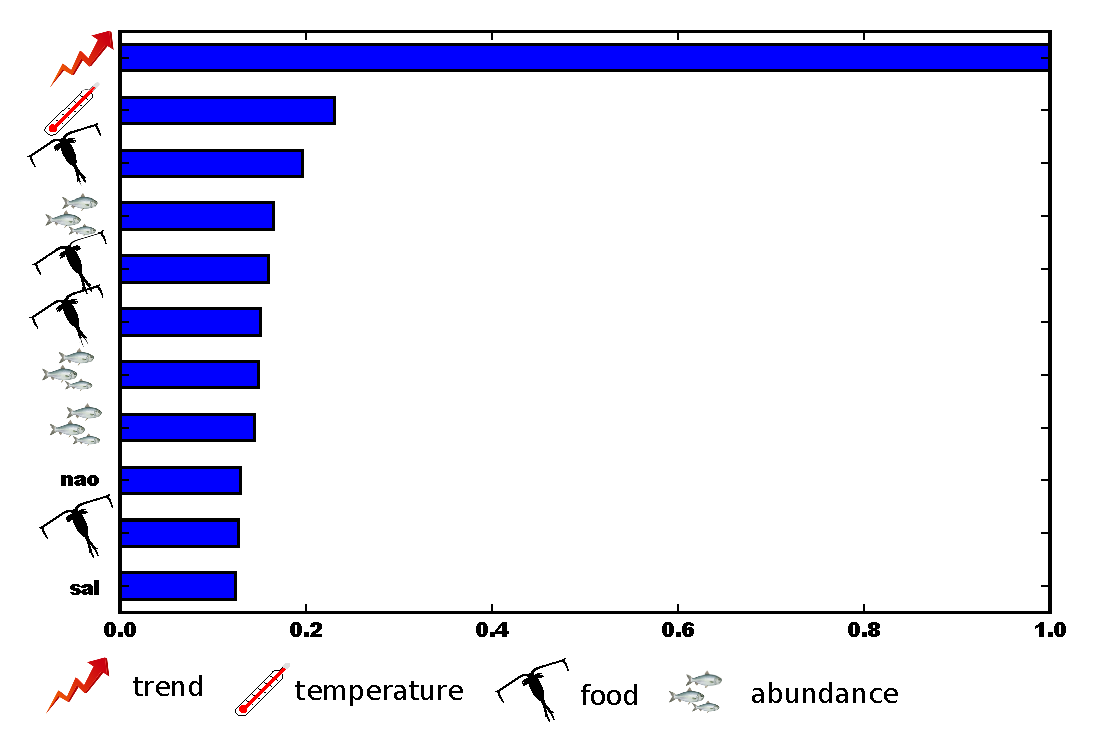
\includegraphics[scale=0.55]{../fig/featureCS-present}
\end{frame}

% Partial dependence plots (PDP) show the dependence between the target response and a set of (‘target’) variables (features), marginalizing over the values of all other features (the ‘complement’ features). 
% Intuitively, we can interpret the partial dependence as the expected target response as a function of the ‘target’ features.
% Partial dependence plots with two target features enable us to visualize interactions among them. 
% ticks are deciles of the input variables

\begin{frame}
\frametitle{Partial Dependence Plots}
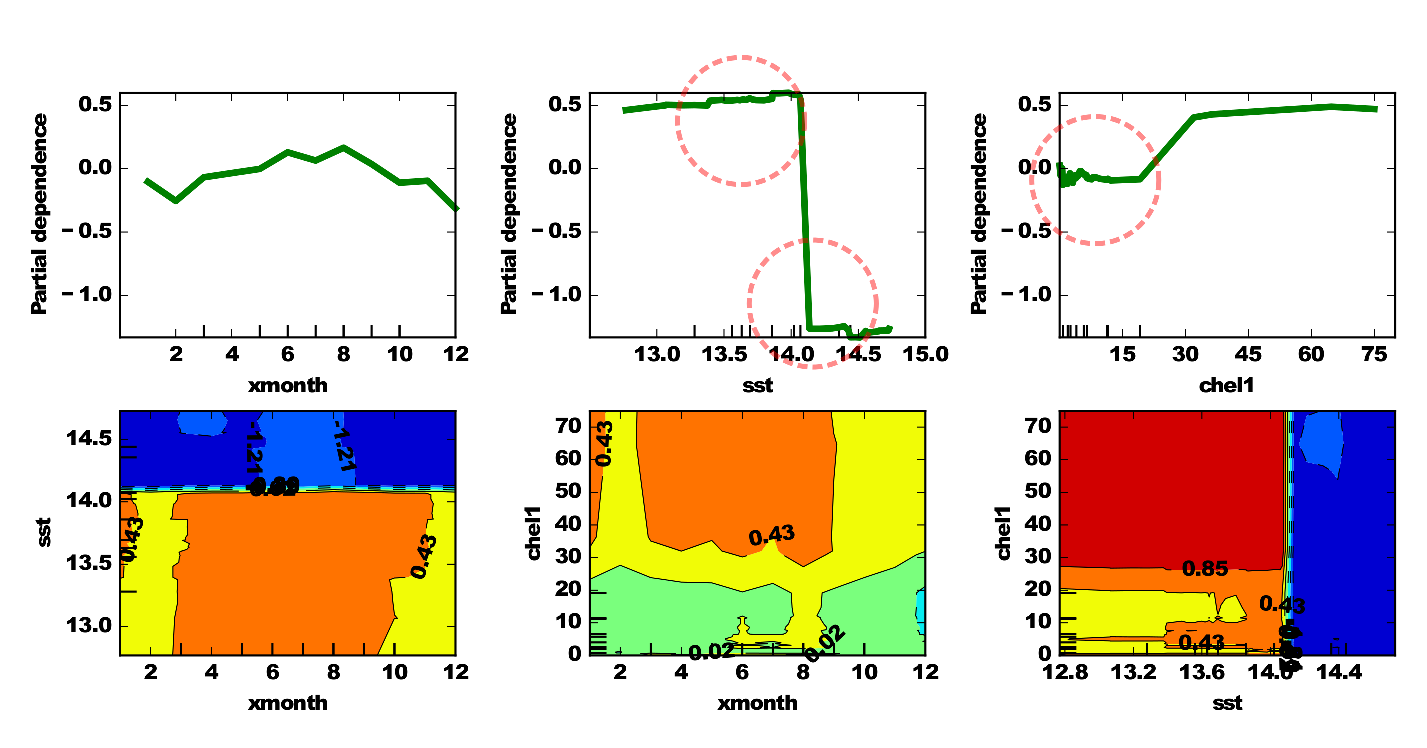
\includegraphics[scale=0.47]{../fig/partdepCS-present}
\end{frame}
% sst and totaln have a strong interaction effect, whereas totaln and recr not as much

\begin{frame}
\frametitle{Conclusions}
\begin{itemize}
    \item <+-| alert@+> trend, sea surface temperature and food availability are three most importans features;
    \item <+-| alert@+> sea surface temperature above 14 degrees negatively relates to fish length, whereas food availability is invariant; %food is not a limiting factor
    \item <+-| alert@+> there is a high degree of interaction between all features;
    \item <+-| alert@+> not a cause-effect relationship, but a relative importance of the variables;
        %low R2 due to individual variability or missing variables..
\end{itemize}
\end{frame}


\begin{frame}
\begin{columns}[c]    
\column{.35\textwidth}
\vspace{1cm}
    \flushleft\raisebox{-0.35ex}{
\includegraphics[width=2.5ex]{../fig/linkedin}}%
    linked.in/lyashevska
    \\
\vspace{-1cm}
    \raisebox{-0.35ex}{
\includegraphics[width=2.5ex]{../fig/github}}%
    lyashevska
\vspace{0.5cm}
\column{.45\textwidth}
\begin{figure}
    
\includegraphics[width=4.5cm]{../fig/logos}
\end{figure}
\end{columns} 

\tiny Acknowledgements: \\

This research was carried out with the support of the Irish Environmental Protection Agency grant (Ecosystem tipping points: learning from the past to manage for the future, project code 2015-NC-MS-3) and the support of the Marine Institute under the Marine Research Sub-programme funded by the Irish Government.  \\
\end{frame}

%\begin{frame}[allowframebreaks]
%\frametitle{References}
%\def\newblock{\hskip .11em plus .33em minus .07em} % important line
%%\nocite{*}
%\bibliographystyle{humannat}
%\small{
%\bibliography{ref}}
%\end{frame}
%
\end{document}

